\chapter{Équations de bilan du laser et du mécanisme de pompe}
\section{Équation de bilan du laser et équations de Maxwell-Bloch}
Reprenons les équations de Maxwell-Bloch d'un laser
\begin{equation}
\left\{\begin{array}{lll}
\dot {\cal E}(t) &\DS=  - \frac{{{K_c}}}{2}{\cal E} + \frac{{i{\omega _c}}}{{2{\varepsilon _0}}}{\cal P}&\qquad(1)\vspace{2mm}\\
\dot {\cal P}(t) &\DS=  - {\gamma _ \bot }{\cal P} - \frac{i}{\hbar }|{\mu _{21}}{|^2}{\cal D}{\cal E} - i({\omega _a} - {\omega _c}){\cal P}(t)&\qquad(2)\vspace{2mm}\\
\dot {\cal D}(t) &\DS=  - {\gamma _\parallel }({{\cal D}} - {\hat {\cal D}}) - \frac{i}{{2\hbar }}({\cal P}{{\cal E}^*} - {\cal E}{{\cal P}^*})&\qquad(3)
\end{array}\right.
\end{equation}
Les différents temps de vies définissent les \textit{classes} des lasers : $AB$ si la polarisation 
est la plus rapide alors que si le champ est le plus lent, on parlera de la classe $A$. Faisons ici 
l'hypothèse que la polarisation répond très rapidement par rapport à la dynamique de $\mathcal{E}$ 
et $\mathcal{D}$
\begin{equation}
{\gamma _ \bot } \gg {\gamma _\parallel },{K_c}/2
\end{equation}
Considérons $\omega_a=\omega_c$ mais aussi $\omega_L=\omega_c$. La seconde équation de MB (2) devient
\begin{equation}
\dot {\cal P}(t) =  - {\gamma _ \bot }{\cal P} - \frac{i}{\hbar }|{\mu _{21}}{|^2}{\cal D}{\cal E}
\end{equation}
En supposant $\mathcal{E}, \mathcal{D}$ constant
\begin{equation}
{\cal P}(t) = {\cal P}(0){{\rm{e}}^{ - {\gamma _ \bot }t}} - \frac{{i|{\mu _{21}}{|^2}}}{{\hbar {\gamma _ \bot }}}{\cal E}{\cal D}(1 - {{\rm{e}}^{ - {\gamma _ \bot }t}})
\end{equation}
Si $t\gg 1/\gamma$ (équivalent à $\dot{\mathcal{P}}(t)=0$ dans (2)) 
\begin{equation}
{\cal P} =  - \frac{{i|{\mu _{21}}{|^2}}}{{\hbar {\gamma _ \bot }}}{\cal E}{\cal D}
\end{equation}
Il s'agit d'une évolution adiabatique de $\mathcal{P}$ qui garde sa valeurs stationnaire. Remplaçons 
cette dernière expression de $\mathcal{P}$ dans (1)
\begin{equation}
\dot {\cal E}(t) =  - \frac{{{K_c}}}{2}{\cal E} + \frac{{i{\omega _c}}}{{2{\varepsilon _0}}}\left( { - \frac{{i|{\mu _{21}}{|^2}}}{{\hbar {\gamma _ \bot }}}{\cal E}{\cal D}} \right)
\end{equation}
Faisons pareil avec (3)
\begin{equation}
\dot {\cal D}(t) =  - {\gamma _\parallel }({{\cal D}} - {\hat {\cal D}}) - \frac{{|{\mu _{21}}{|^2}}}{{2{\hbar ^2}{\gamma _ \bot }}}2{\cal D}|{\cal E}{|^2}
\end{equation}
Cette expression de l'inversion de population dépend du terme de pompage ainsi que du module carré 
de $\mathcal{E}$. Afin de remplacer l'une dans l'autre, on va multiplier cette expression par son 
conjugué ($\mathcal{E}^*\mathcal{E}=|\mathcal{E}|^2$). Si $\mathcal{I}=|\mathcal{E}|^2$, alors\\

\retenir{
\begin{equation}
\left\{\begin{array}{lll}
{\dot {\cal I}}(t) &\DS=  - {K_c}{{\cal I}} + \frac{{{\omega _c}|{\mu _{21}}{|^2}}}{{\hbar {\gamma _ \bot }{\varepsilon _0}}}{\cal D}{{\cal I}}&\qquad(4)\vspace{2mm}\\
\dot {\cal D}(t) &\DS=  - {\gamma _\parallel }({{\cal D}} - {\hat {\cal D}}) - \frac{{|{\mu _{21}}{|^2}}}{{{\hbar ^2}{\gamma _ \bot }}}{\cal D}{{\cal I}}&\qquad(5)
\end{array}\right.
\end{equation}
Ces deux équations sont connues comme les équations de bilan d'un laser. Elles décrivent la 
dynamique des laser de classes dynamiques $A$ et $B$.}


\section{Systèmes à deux niveaux}
	\begin{wrapfigure}[6]{r}{6cm}
	\vspace{-8mm}
	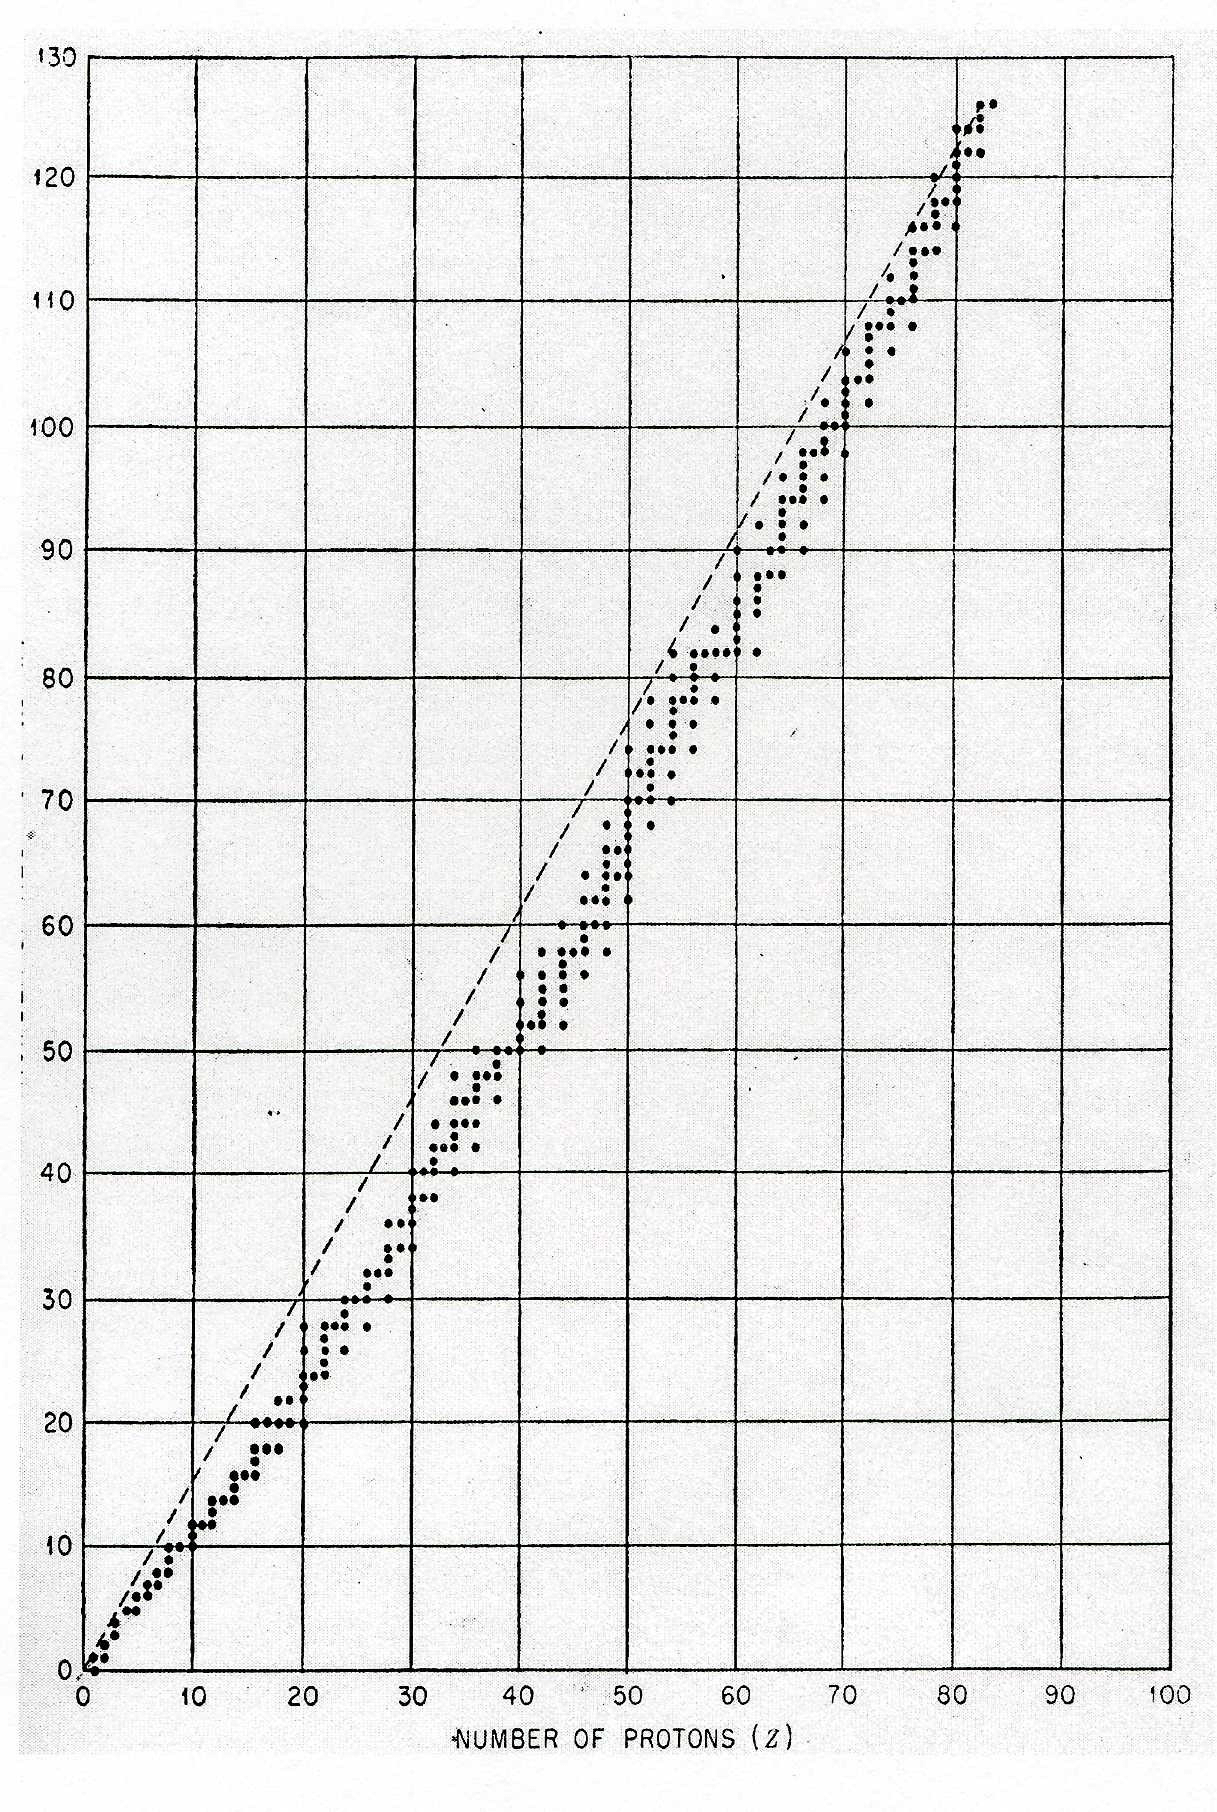
\includegraphics[scale=0.6]{ch4/image1.png}
	\captionof{figure}{ }
	\end{wrapfigure}
Considérons un flux de photon incident dont l'énergie est celle entre deux niveaux. Pour une onde 
monochromatique incidente à $\omega_0$ :
\begin{equation}
u = {n_p}\hbar {\omega _0}\delta (\omega  - {\omega _0}),\qquad 
{{\cal J}} = {n_p}{v_g},\qquad \hbar\omega_a = E_2-E_1
\end{equation}
Il est possible de calculer le taux d'absorption $\DS{\Gamma _{12}} = \int {{B_{12}}u(\omega )g(\omega ){N_1}{\rm{d}}\omega }$ en y remplaçant $u$ monochromatique 
\begin{equation}
{\Gamma _{12}} = \sigma {{\cal J}}{N_1}
\end{equation}
où $\DS \sigma  = B\hbar {\omega _0}g({\omega _0})/{v_g}$ est la section efficace ($m^2$). Le taux 
de variation de la population atomique s'exprime
\begin{equation}
{\dot N_2} = {\Gamma _{12}} - {\Gamma _{21}} - {T_{21}}{N_2},\qquad
{\dot N_1} =  - ({\Gamma _{12}} - {\Gamma _{21}}) + {T_{21}}{N_2}
\end{equation}
où ${T_{21}} = {A_{21}} + {S_{21}}$ (le premier est radiatif, pas le second)\footnote{Qu'est ce que 
ça représente exactement?}. En en tire
\begin{equation}
\frac{{\rm{d}}}{{{\rm{d}}t}}({N_1} + {N_2}) = 0 \Rightarrow {N_1} + {N_2} = N
\end{equation}
Pour la solution stationnaire (par exemple $\dot{N_2}=0$)
\begin{equation}
\sigma {{\cal J}}({N_1} - {N_2}) = {T_{21}}{N_2}
\end{equation}
Sachant que $\mathcal{D}=N_2-N_1\leftrightarrow \mathcal{D}+N=2N_2$ 
\begin{equation}
 - \sigma {{\cal J}{\cal D}} = {T_{21}}({{\cal D}} + N)/2\qquad\Rightarrow\qquad
{{\cal D}} =  - N\frac{1}{{1 + 2\sigma {{\cal J}}/{T_{21}}}}
\end{equation}
Cette expression est logique car s'il n 'y a pas de courant on trouve $\mathcal{D}=-N$ : on ne peut 
pas avoir d'inversion de population car $\mathcal{D}$ est toujours négatif.\\

Explicitons cette expression de l'inversion de population. Nous savons (en substituant les expressions 
terme à terme) que
\begin{equation}
2\sigma {{\cal J}}/{T_{21}} = 2\frac{{B\hbar {\omega _0}g({\omega _0})}}{{{v_g}}}\frac{I}{{\hbar {\omega _0}}}/{T_{21}} = \frac{I}{{{I_s}}}\tilde g({\omega _0})
\end{equation}
où $\tilde g({\omega _0}) = \frac{{g({\omega _0})}}{{g({\omega _a})}}$. L'\textbf{intensité de 
saturation} est définie comme ($W.m^{-2}$)
\begin{equation}
{I_s} = \frac{{{v_g}{T_{21}}}}{{2Bg({\omega _a})}}
\end{equation}
On arrive alors à ré-écrire $\mathcal{D}$
\begin{equation}
{{\cal D}} =  - N/[1 + \frac{I}{{{I_s}}}\tilde g({\omega _0})]
\end{equation}
Comme $\mathcal{D}<0$, cela montre qu'il n'est pas possible d'atteindre l'inversion de population 
dans un régime stationnaire ($\alpha = -\sigma\mathcal{D} > 0$, pas de gain). 
\begin{center}
	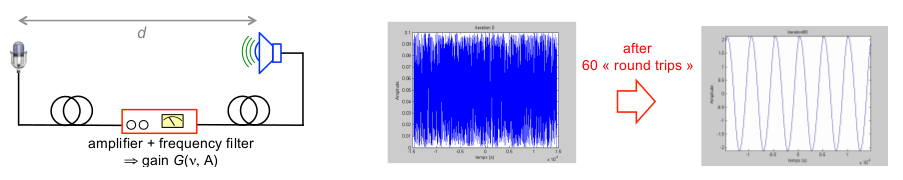
\includegraphics[scale=0.6]{ch4/image2.png}
	\captionof{figure}{ }
\end{center}
Considérons le cas 
d'une absorption
\begin{equation}
\frac{{\rm{d}}}{{{\rm{d}}z}}I =  - \alpha I
\end{equation}
où $\DS\alpha  =  - \sigma {{\cal D}} = \sigma N/[1 + \frac{I}{{{I_s}}}\tilde g({\omega _0})]$. 
Passons en revue deux cas 
\begin{enumerate}
\item $I\ll I_s$ (absorption non saturée)
\begin{equation}
\alpha\approx \sigma N \qquad \Rightarrow\qquad I(z) = {I_0}{\rm{exp(}} - \sigma Nz{\rm{)}}
\end{equation}
A faible intensité (par rapport à celle de saturation) il y a donc beaucoup d'absorption
\begin{center}
	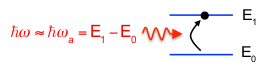
\includegraphics[scale=0.6]{ch4/image3.png}
	\captionof{figure}{ }
\end{center}


\item $I \gg I_s$ (absorption saturée)
\begin{equation}
\alpha  \approx \sigma N\frac{{{I_s}}}{I}\qquad\Rightarrow\qquad 
I(z) = {I_0} - {I_s}\sigma Nz
\end{equation}
Lorsque l'on atteint une intensité proche de celle de saturation, on observe une décroissance 
linéaire de l'intensité ce qui est une grosse différence. On parle de \textit{transparence 
auto-induite}\footnote{Heu..?}
\begin{center}
	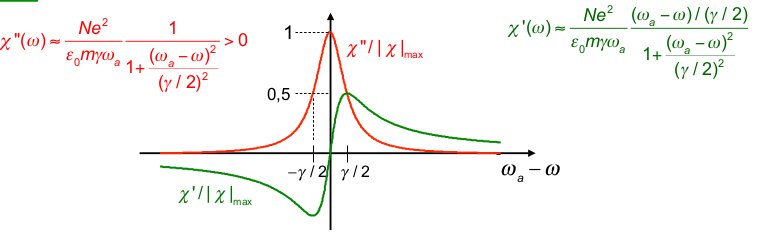
\includegraphics[scale=0.6]{ch4/image4.png}
	\captionof{figure}{ }
\end{center}
\end{enumerate}

Même si ce système a deux niveau, il n'est pas utile pour en faire un laser (car $\mathcal{D}<0$) 
mais on peut l'utiliser pour générer de courtes impulsions. Pour avoir un gain dans le système 
($\mathcal{D}>0$) il faut un système atomique avec plus de deux niveaux (au moins 
trois ou autre niveaux d'énergie participant au lasage/pomapge).

\section{Laser à trois niveaux d'énergie}
	\begin{wrapfigure}[7]{l}{6cm}
	\vspace{-5mm}
	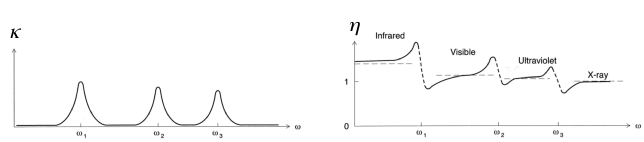
\includegraphics[scale=0.6]{ch4/image5.png}
	\captionof{figure}{ }
	\end{wrapfigure}
Pour contrer ce problème, nous allons utiliser un niveau de plus haute énergie dont le but est de 
nourrir le second niveau et non pas que deux niveau qui se peuplent et dépeuplent. L'idée est de 
s'arranger pour que le taux de $3\to1 \ll 3\to 2$. Nous allons ici considérer un système Er (erbium) 
à trois niveaux. La densité totale est la somme des densités de chaque niveau.
\begin{equation}
N= N_1+N_2+N_3\qquad (6)
\end{equation}
Comme annoncé, on fait l'hypothèse que le niveau 3 se désexcite préférentiellement vers le second 
niveau et non pas le fondamental
\begin{equation}
T_{31}N_3 \ll T_{32}N_3
\end{equation}
Soit $W_p=\sigma_p\mathcal{J}_p$ ($s^{-1}$) le taux de pompage optique. Étudions la variation de 
densité du niveau trois
\begin{equation}
{\dot N_3} = {W_p}{N_1} - {W_p}{N_3} - {T_{32}}{N_3}\qquad(7)
\end{equation}
Il s'agit de la contribution de la pompe, mais aussi l'émission stimulée $3\to1$ du à la pompe et 
aux transitions\footnote{Expliciter}. De même pour le niveau 2
\begin{equation}
{\dot N_2} =  + {T_{32}}{N_3} - ({N_2} - {N_1})\sigma {{\cal J}} - {T_{21}}{N_2}
\end{equation}
Il peut être peuplé depuis le niveau 3, il peut avoir de l'émission stimulée, de l'absorption et 
$T_{21}N_1$ l'émission stimulée de $2\to1$. En faisant de même pour le niveau fondamental
\begin{equation}
{\dot N_1} = ({N_2} - {N_1})\sigma {{\cal J}} + {T_{21}}{N_2} - {W_p}({N_1} - {N_3})
\end{equation}
En faisant un peu de mathématiques (non détaillées ici) on peut obtenir une équation donnant le 
rapport entre l'inversion de population et la densité totale
\begin{equation}
\frac{{{\cal D}}}{N} = \frac{{{W_p}({T_{32}} - {T_{21}}) - {T_{21}}{T_{32}}}}{{3\sigma {{\cal J}}{W_p} + 2{W_p}{T_{21}} + 2\sigma {{\cal J}}{T_{32}} + {T_{21}}{T_{32}} + {W_p}{T_{32}}}}
\end{equation}
Le dénominateur n'a que des signes positif. S'il n'y a pas de pompe, le rapport est négatif et on 
n'a pas d'inversion de population (ce qui est cohérent). Pour avoir une inversion, il faut que $T_{32}
\gg T_{21}$ ce qui signifie que le temps de désexcitation de $2\to3$ doit être plus petit que 
$2\to1$.\\

On peut définir un taux de pompage de transparence (autant d'absorption que d'émission stimulée, dès 
qu'un photon descend dans le niveau 1, un autre remonte directement dans le niveau 3). 
\begin{equation}
W_p^{t - th} = {T_{21}}{T_{32}}/({T_{32}} - {T_{21}})
\end{equation}
Pour obtenir ce milieu transparent, il faut que $T_{32}\gg T_{21} \Rightarrow W_p^{t - th} \approx {T_{21}}$. \\

Faisons cette supposition de milieu transparent impliquant une élimination adiabatique en $N_3$. Après 
quelques substitutions (slide 8)
\begin{equation}
{\dot {\cal D}} = 2{W_p}(N - {{\cal D}})/2 - 2{{\cal D}}\sigma {{\cal J}} - 2{T_{21}}(N + {{\cal D}})/2 =  - ({W_p} + {T_{21}}){{\cal D}} - 2{{\cal D}}\sigma {{\cal J}} + ({W_p} - {T_{21}})N
\end{equation}
La dernière égalité est formellement égale à
\begin{equation}
\dot {\cal D}(t) =  - {\gamma _\parallel }({{\cal D}} - {\hat {\cal D}}) - \frac{{|{\mu _{21}}{|^2}}}{{{\hbar ^2}{\gamma _ \bot }}}{\cal D}{{\cal I}}
\end{equation}

	\begin{wrapfigure}[9]{l}{6cm}
	\vspace{-12mm}
	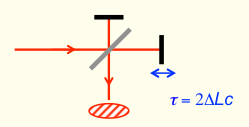
\includegraphics[scale=0.6]{ch4/image6.png}
	\captionof{figure}{Si pompage trop faible : gain négatif $\to$ pertes}
	\end{wrapfigure}
On trouve une valeur du coefficient de relaxation qui dépend de $T_{21}$ mais aussi du taux de 
pompage ce qui peut ne pas paraître évident. Tout se réparti donc entre le niveau fondamental et le 
second niveau, le niveau 3 n'est qu'une "étape nécessaire" pour atteindre le second niveau.\\

Regardons la solution stationnaire au dessus, en dessous et au seuil laser\\

\begin{itemize}
\item[$\bullet$] En dessous du seuil laser $\mathcal{J}=0$
\begin{equation}
{{\cal D}} = \frac{{({W_p} - {T_{21}})}}{{({W_p} + {T_{21}})}}N = {\hat {\cal D}}
\end{equation}
Lorsque $W_p > W_p^{t-th}, \mathcal{G}=\sigma\mathcal{D}$ et l'on retrouve un amplification 
exponentielle.
\item[$\bullet$] Au seuil laser.
\begin{equation}
{{{\cal G}}_s} = \sigma {{{\cal D}}_s} = {K_c}/c\qquad\Rightarrow\qquad 
W_p^{l - th} = {T_{21}}\frac{{1 + {K_c}/Nc\sigma }}{{1 - {K_c}/Nc\sigma }} > {T_{21}} = W_p^{t - th}
\end{equation}
On observe une diminution de la transparence $W$ si $T_{21}$ et $K_c$ diminuent.
\item[$\bullet$] Au dessus du seuil laser : $\mathcal{J}\neq0$
\begin{equation}
{{\cal D}} = \frac{{({W_p} - {T_{21}})/({W_p} + {T_{21}})}}{{1 + 2\sigma {{\cal J}}/({W_p} + {T_{21}})}}N
\end{equation}
Ceci correspond à la saturation de l'inversion de population : $\mathcal{D}=\mathcal{D}_s=c^{te}$.
\end{itemize}
En résumé, on augmente $W_p$ jusqu'au seuil de transparence où l'on commence à obtenir du gain. En 
continuant d'augmenter le laser démarre jusqu'à arriver à quelque chose de constant. On peut voir 
que ce taux diminue si $T_{21}$ : si tous les atomes restaient en $N2$ sans redescendre en $N1$ ce 
serait effectivement génial mais forcement ce n'est pas réalisable et on perd des photons dans une
fluorescence inutile. Si l'on regarde le graphe $W_p\propto P$ en fonction de $z$ on voit qu'à partir
d'une certaine longueur la fibre devient absorbante!




\newpage
\section{Laser à quatre niveaux d'énergie}
	\begin{wrapfigure}[9]{r}{7cm}
	\vspace{-8mm}
	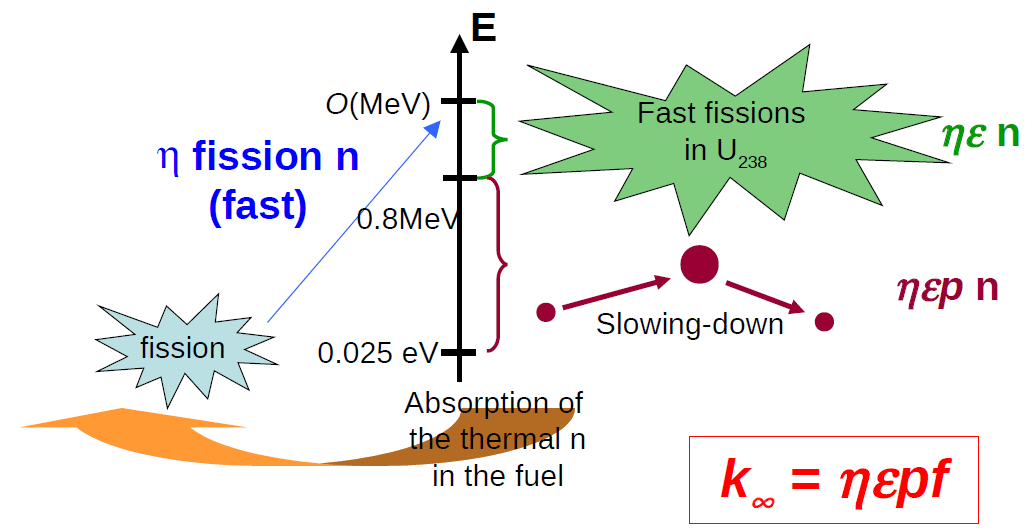
\includegraphics[scale=0.6]{ch4/image7.png}
	\captionof{figure}{ }
	\end{wrapfigure}
Le but d'un tel système est de surmonter le problème des lasers à trois niveaux qui nécessite de
monter plus de la population atomique dans l'état supérieur pour avoir un gain $\mathcal{G}>0$. Les 
équations sont semblables à celles à trois niveau
\begin{equation}
\begin{array}{ll}
N &= {N_1} + {N_2} + {N_3} + {N_4}\\
{\dot N_4} &= {W_p}({N_1} - {N_4}) - {T_{43}}{N_4}\\
{\dot N_3} &=  - \sigma {{\cal J}}({N_3} - {N_2}) + {T_{43}}{N_4} - {T_{32}}{N_3}\\
{\dot N_2} &=  + \sigma {{\cal J}}({N_3} - {N_2}) + {T_{32}}{N_3} - {T_{21}}{N_2}\\
{\dot N_1} &=  - {W_p}({N_1} - {N_4}) + {T_{21}}{N_2}
\end{array}
\end{equation}
Par exemple, pour $\dot{N_2}$ on retrouve le terme de désexcitation stimulée $3\to 2$, l'excitation 
spontannée radiative (ou non) de $3\to 2$ ($T_{32}N_3$), la diminution due à une désexcitation 
spontannée ($T_{21}N_2$) et enfin on peut avoir de l'absorption ($-\sigma N_2$).\\

Il est important que $T_{43}$ soit rapide\footnote{Et donc très grand de sorte que le temps de vie soit très court} et $T_{43}\gg W_p$. La transition laser se fera entre le niveau 3 et 2 et du 2 il
retombera dans le fondamental. Il est aussi nécessaire que le niveau 2 ne soit pas rempli par excitation thermique ($E_1-E_2\gg k_BT$)  sinon cela ressemble plus à un système à trois niveaux
\begin{equation}
\dfrac{N_2}{N_1} = e^{-(E_2-E_1)/k_BT} \ll 1
\end{equation}
Cette décroissance rapide de $4\to3$ est l'\textit{élimination adiabatique} de $N_4$
\begin{equation}
({W_p} + {T_{43}}){N_4} = {N_1}{W_p} \approx {T_{43}}{N_4} \Rightarrow {N_4} \approx 0
\end{equation}
Intéressons-nous à la solution stationnaire
\begin{equation}
\left.\begin{array}{ll}
{N_1}{W_p} &= {T_{21}}{N_2}\\
N &= {N_1} + {N_2} + {N_3} \Rightarrow {N_3} = N - {N_2}(1 + {T_{21}}/{W_p})
\end{array}\right\}\Rightarrow {{\cal D}} \equiv {N_3} - {N_2} \Rightarrow {N_2} = 
\dfrac{N-\mathcal{D}}{2 + {T_{21}}/{W_p}}
\end{equation}
Avec l'expression de $\dot{N_3}$, celle de $N_3$ que nous venons d'obtenir et de même pour 
$\mathcal{D}$, on peut écrire
\begin{equation}
{{\cal D}}/N = \frac{{{W_p}({T_{21}} - {T_{32}})}}{{\sigma {{\cal J}}(2{W_p} + {T_{21}}) + {W_p}
({T_{32}} + {T_{21}}) + {T_{32}}{T_{21}}}}
\end{equation}
Nous voulons que l'inversion de population soit positive sans quoi il n'y aura jamais de laser et
l'espèce atomique sera à rejeter. Le dénominateur étant toujours positif, le signe de l'inversion 
de population dépend du signe de cette fraction. Pour que ce soit le cas, il faut que $T_{21}>
T_{32}$ : la descente doit se faire plus vite de $2\to 1$ que de $3\to2$ car on souhaite qu'un 
maximum d'atome reste en 3. Si un des atomes redescend comme on souhaite éviter l'accumulation en 2
il faudrait qu'il redescende directement en 1 (pour éviter l'absorption de $2\to 3$).\\

Supposons $T_{21}\gg T_{32}$. Ceci implique l'élimination de $N_2$ dans l'expression de $\dot{N_2}$
\begin{equation}
{\dot N_2} =  + \sigma {{\cal J}}({N_3} - {N_2}) + {T_{32}}{N_3} - {T_{21}}{N_2}\Rightarrow
\sigma {{\cal J}{\cal D}} + {T_{32}}{N_3} = {T_{21}}{N_2}
\end{equation}
Et donc
\begin{equation}
{N_2} = (\sigma {{\cal J}{\cal D}} + {T_{32}}{N_3})/{T_{21}} \approx 0 \Rightarrow N \approx {N_1} + {N_3}
\end{equation}
Comme nous avons $N \approx {N_1} + {N_3}$ et  ${{\cal D}} = {N_3} - {N_2} \approx {N_3}$, on tire
avec l'équation de $\dot{N_3}$
\begin{equation}
{\dot {\cal D}} = {\dot N_3} =  - \sigma {{\cal J}{\cal D}} + {W_p}{N_1} - {T_{32}}{N_3}
\end{equation}
Sachant que $N_3\approx\dot{D}$ et $N_1=N-N_3$
\begin{equation}
{\dot {\cal D}} =  \underbrace{- ({W_p} + {T_{32}}){{\cal D}}}_{-\gamma_\perp\mathcal{D}} - \sigma {{\cal J}{\cal D}} + \underbrace{{W_p}N}_{\gamma_\parallel\hat{\mathcal{D}}}
\label{eq:Ch4.17}
\end{equation}
Cette équation à une forme similaire à celle précédemment obtenue:
\begin{equation}
\dot {\cal D}(t) =  - {\gamma _\parallel }({{\cal D}} - {\hat {\cal D}}) - \frac{{|{\mu _{21}}{|^2}}}{{{\hbar ^2}{\gamma _ \bot }}}{\cal D}{{\cal I}}
\end{equation}
Étudions la solution stationnaire de \eqref{eq:Ch4.17}
\begin{itemize}
\item[$\bullet$] En dessous du seuil laser $\mathcal{J}=0$
\begin{equation}
{{\cal D}} = {\hat {\cal D}} = [{W_p}/({W_p} + {T_{32}})]N > 0
\end{equation}
Si pas de pompage, c'est forcément nul. Lorsque l'on pompe, de l'accumulation se 
forme en 3 et il y aura directement du gain car les constantes sont bien choisies. Si l'on ne se 
trouve pas dans une cavité $N_3$ augmentera au maximum jusqu'à $N$ mais pour un laser il y en a une. 
L'inversion de population tel que gain=pertes  va faire démarrer le laser à $\mathcal{D}=\mathcal{D}_s$
\item[$\bullet$] Au seuil laser
\begin{equation}
{{{\cal G}}_s} = \sigma {{{\cal D}}_s} = {K_c}/c\quad\Rightarrow\quad 
W_p^{sl} = \frac{{{T_{32}}{K_c}}}{{N\sigma c - {K_c}}}
\end{equation}
Le numérateur est positif si $N\sigma c>K_c$. Plus $K_c$ est faible, plus la condition pertes=gain 
est facile à obtenir
\end{itemize}
\begin{center}
	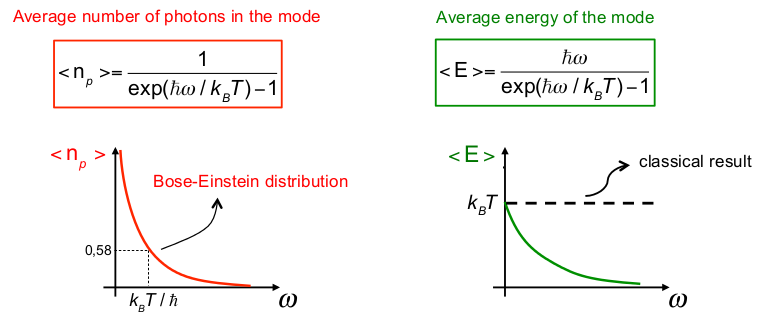
\includegraphics[scale=0.6]{ch4/image8.png}
	\captionof{figure}{L'inversion n'est ici jamais négative, il n'y a pas de risque d'introduire des
	pertes en pompant trop peu.}
\end{center}

Notons que les laser $CO_2$ sont des lasers à trois niveaux mais suivent les mêmes équations que les
lasers à 4 niveaux\footnote{Lire illustration notes personnelles slide 15.}.

\newpage
\section{Rendement laser}
Le but de cette section est de déterminer les points critiques qui vont faire en sorte que le 
rendement soit très important ou très faible. Le rendement d'un laser suit bien évidemment la définition standard
\begin{equation}
{\eta _l} \equiv \frac{{{\rm{Output laser power}}}}{{{\rm{Pump power}}}} = \frac{{{P_{{\rm{out}}}}}}{{{P_{{\rm{in}}}}}}
\end{equation}
Par simplicité au niveau des conversions, on va supposer que le pompage est optique. La puissance 
de sortie est liée à la fraction quittant la cavité
\begin{equation}
1/{t_c} = {\alpha _i}c - (c/L)\ln ({R_1}) = {\alpha _i}c + {\alpha _m}c = {\alpha _c}c
\end{equation}
où $- (c/L)\ln ({R_1})$ sont les pertes dues aux miroirs. On les note généralement $-\alpha_m$ mais 
il faut bien gardé que ce sont des pertes utiles contrairement à $\alpha_i$, les pertes internes. 
Le taux de photons quittant la cavité par le coupleur de sortie (miroir 1) est donné par\begin{equation}
\alpha_m.c.N_p
\end{equation}
où $N_p$ est le nombre de photons dans la cavité. On peut l'écrire
\begin{equation}
{{\rm{N}}_p} = {n_{\rm{p}}}AL
\end{equation}
où $n_p$ est la densité de photon dans la cavité, $AL$ le volume occupé par les photons (mode laser) 
dans la cavité avec $A$ la "surface transverse" du mode laser. L'intensité sortant s'écrit 
\begin{equation}
{P_{{\rm{out}}}} = {\alpha _m}c{n_{\rm{p}}}AL\hbar {\omega _L}
\end{equation}
Il est plus intéressant d'écrire l'intensité de la cavité en terme de flux. C'est faisable sachant 
que la densité de photon peut s'écrire\footnote{$\mathcal{J}_L$ est approximée au-delà du seuil 
laser.}
\begin{equation}
{n_{\rm{p}}} = {{{\cal J}}_L}/c\qquad\text{où }\quad {{{\cal J}}_L} = {{{\cal J}}_s}\left(\frac{{{\hat {\cal D}}}}{{{{{\cal D}}_s}}} - 1\right) \approx {{{\cal J}}_s}\frac{{{\hat {\cal D}}}}{{{{{\cal D}}_s}}}
\end{equation}
En outre, la condition d'oscillation laser étant ${\sigma _L}{{{\cal D}}_s} = {K_c}/c = {\alpha _c}$, 
on peut ré-écrire $\mathcal{J}_L$
\begin{equation}
{{{\cal J}}_L} = \underbrace{{\sigma _L}{{{\cal J}}_s}}_{?}\frac{{{\hat {\cal D}}}}{{{\alpha _c}}}
\end{equation}
Il faut essayer d'exprimer ce point d'interrogation. Pour se faire, nous allons comparer l'équation 
de bilan obtenue via Maxwell-Bloch et celle obtenue pour le système à 4 niveaux
\begin{equation}
\dot {\cal D}(t) =  - {\gamma _\parallel }({{\cal D}} - {\hat {\cal D}}) -\underbrace{\frac{{|{\mu _{21}}{|^2}}}{{{\hbar ^2}{\gamma _ \bot }}}{\cal D}{{\cal I}}}_{(*)},\qquad {\dot {\cal D}} =  - ({W_p} + {T_{32}}){{\cal D}} - \underbrace{\sigma {{\cal J}{\cal D}}}_{(*)} + {W_p}N
\end{equation}
On s'intéresse aux termes\footnote{Je vois pas en quoi.} $(*)$. En remplaçant$\sigma_L\mathcal{J}_s$
par sa définition (et avec la définition de $\mathcal{I}_s$)
\begin{equation}
{\sigma _L}{{{\cal J}}_s} = \frac{{|{\mu _{21}}{|^2}}}{{{\hbar ^2}{\gamma _ \bot }}}{{{\cal I}}_s}
\qquad\text{où }\quad {{{\cal I}}_s} = \frac{{{\hbar ^2}{\gamma _\parallel }{\gamma _ \bot }}}{{|{\mu _{21}}{|^2}}}
\end{equation}
Ceci implique que
\begin{equation}
\Rightarrow {\sigma _L}{{{\cal J}}_s} = \frac{{|{\mu _{21}}{|^2}}}{{{\hbar ^2}{\gamma _ \bot }}}\frac{{{\hbar ^2}{\gamma _\parallel }{\gamma _ \bot }}}{{|{\mu _{21}}{|^2}}} = {\gamma _\parallel }
\end{equation}
On peut\footnote{Comment?} en déduire $\mathcal{J}_L$
\begin{equation}
{{{\cal J}}_L} = {\sigma _L}{{{\cal J}}_s}\frac{{{\hat {\cal D}}}}{{{\alpha _c}}} = \underbrace{{\gamma _\parallel }{\hat {\cal D}}}_{W_pN}/{\alpha _c}
\end{equation}
On en tire la puissance de sortie
\begin{equation}
{P_{{\rm{out}}}} = {\alpha _{\rm{m}}}\hbar {\omega _L}c\frac{{{{{\cal J}}_L}}}{c}AL = \frac{{{\alpha _{\rm{m}}}}}{{{\alpha _{\rm{c}}}}}\hbar {\omega _L}{W_p}NAL
\end{equation}
Il ne reste que la puissance d'entrée à considérer. La puissance qui rentre c'est l'énergie par unité 
dans la cavité soit le flux de photon * l'énergie * aire transverse de pompage
\begin{equation}
{P_{{\rm{in}}}} = \hbar {\omega _p}{{{\cal J}}_p}{A_p}
\end{equation}
où ${\sigma _p}{{{\cal J}}_p} = {W_p}$. Le \textbf{rendement} s'exprime alors
\begin{equation}
{\eta _l} = \frac{{{P_{{\rm{out}}}}}}{{{P_{{\rm{in}}}}}} = \frac{{\hbar {\omega _L}}}{{\hbar {\omega _p}}}\frac{{{\alpha _{\rm{m}}}}}{{{\alpha _{\rm{c}}}}}\frac{A}{{{A_p}}}{\sigma _p}NL = {\eta _q}{\eta _d}{\eta _t}{\eta _a}
\end{equation}
\begin{description}
\item[$\eta_q$] il s'agit du \textit{rendement quantique} : un photon absorbé doit donné un photon 
laser. Nous avions vu dans les laser à 4 niveaux qu'il devait être supérieur à l'énergie du laser, 
mais si celui-ci est trop grand on perd pas mal.
\item[$\eta_d$] il s'agit du \textit{rendement de couplage}: ce sont les pertes utiles. On serait 
tenté de mettre un mauvais coupleur pour faire tendre ce facteur vers l'unité mais le souci c'est 
que si on fait ça, il y aura plus de pertes et pour attendre perte = gain il faudra plus pomper : 
compromis.
\item[$\eta_t$] il s'agit du \textit{rendement transverse} (recouvrement spatial) : il tend vers 
zéro si l'aire de pompage est grande devant l'aire occupée par les photons laser. L'idéeal c'est 
d'avoir un mode laser large avec un pompage plus petit
\item[$\eta_a$] il s'agit du \dots Mystère et boule de gomme!
\end{description}

Essayons d'interpréter $\eta_a$. Commençons par faire l'hypothèse d'un taux de pompage faible tel
que $N \approx N_1$ (ce n'est pas un problème car dès qu'il y a des atomes en $N_3$ il y a du gain). On suppose également que le milieu à gain est très petit de sorte à supposer que le gain est 
constant (on est obligé de faire ça car la variable $z$ à disparue des équations par changement de 
variables). 
\begin{equation}
\frac{{{\rm{d}}{N_1}}}{{{\rm{d}}t}} =  - {\sigma _p}{{{\cal J}}_p}N =  - {\sigma _p}{n_{pp}}cN = \frac{{{\rm{d}}{n_{pp}}}}{{{\rm{d}}t}}
\end{equation}
où $n_{pp}$ est la densité de photons de pompe. En divisant par le temps, il est possible de retrouver
ce fameux $\eta_a$
\begin{equation}
\frac{{\Delta {n_{pp}}}}{{\Delta t}} = c\frac{{\Delta {n_{pp}}}}{L} =  - {\sigma _p}{n_{pp}}cN\qquad
\Rightarrow\qquad \Delta {n_{pp}}/{n_{pp}} =  - {\sigma _p}NL
\end{equation}
Le rendement $\eta_a$ est donc le rendement d'absorption de la pompe. Dans un cas plus réaliste, il 
faut tenir compte de la décroissance de l'amplitude avec $z$. En supposant un faisceau gaussien 
(bonne hypothèse), le rendement transverse vaut ${\eta _t} = \frac{A}{{A + {A_p}}}$ et on en tire
\begin{equation}
{\eta _a} = 1 - \exp ( - \alpha L)
\end{equation}
où $\alpha = \sigma_p(N_1-N_2) \approx\sigma_pN$. Le rendement laser vaut donc bien\\

\cadre{
\begin{equation}
{\eta _l} = {\eta _q}{\eta _d}{\eta _t}{\eta _a}
\end{equation}}\ \\

Pour le maximiser, il faut
\begin{itemize}
\item[$\bullet$] Minimiser les pertes internes par rapport à celles du coupleur
\item[$\bullet$] Maximiser l'absorption de la pompe
\item[$\bullet$] Optimiser le recouvrement spatial dans le milieu à gain
\item[$\bullet$] Faible différence d'énergie entre $\hbar\omega_p$ et $\hbar\omega_L$
\end{itemize}















